\documentclass[letterpaper,10pt]{article}
\usepackage[utf8]{inputenc}
\usepackage[spanish,es-lcroman]{babel}
\usepackage{amsfonts}
\usepackage{amsmath}
\usepackage{graphicx}
\usepackage{url}
\usepackage[top=3cm,bottom=3cm,left=3.5cm,right=3.5cm,footskip=1.5cm,headheight=1.5cm,headsep=.5cm]{geometry}
\usepackage{multirow}
\usepackage{float}
\usepackage{booktabs}
\usepackage{algorithm}
\usepackage{algpseudocode}
% \usepackage{biblatex}

\renewcommand{\arraystretch}{1.2}

\begin{document}

\title{Inteligencia Artificial \\
 \begin{Large}Informe Final: Balanced Academic Curriculum Problem\end{Large}}


\author{Juan Pablo Escalona G.}


\date{\today}

\maketitle


%--------------------No borrar esta secci\'on--------------------------------%


\section*{Evaluación}

\begin{tabular}{ll}
Mejoras 1ra Entrega (10 \%):  & \underline{\hspace{2cm}}\tabularnewline
Código Fuente (10 \%):  & \underline{\hspace{2cm}}\tabularnewline
Representación (15 \%):  & \underline{\hspace{2cm}} \tabularnewline
Descripción del algoritmo (20 \%):  & \underline{\hspace{2cm}} \tabularnewline
Experimentos (10 \%):  & \underline{\hspace{2cm}} \tabularnewline
Resultados (10 \%):  & \underline{\hspace{2cm}} \tabularnewline
Conclusiones (20 \%):  & \underline{\hspace{2cm}}\tabularnewline
Bibliograf\'{i}a (5 \%):  & \underline{\hspace{2cm}}\tabularnewline
 & \tabularnewline
\textbf{Nota Final (100)}:  & \underline{\hspace{2cm}} \tabularnewline
\end{tabular}%---------------------------------------------------------------------------%
\vspace{2cm}
\begin{abstract}
% Resumen del informe en no más de 10 líneas, donde se sintetice el
% problema que se trata y sirva para que un lector no involucrado comprenda
% el objetivo del documento. \textbf{Además, debería tener una pequeña
% síntesis del acercamiento que se utiliza en cada trabajo, con los
% resultados más destacables o logros en los experimentos realizados.}
Balanced Academic Curriculum Problem, también llamado BACP,
es un problema que busca asignar los ramos de una malla curricular
en diferentes periodos de manera balanceada para que los alumnos
puedan cursar exitosamente los ramos dependiendo de la carga (cr\'editos)
de estos, cumpliendo restricciones asociadas al la cantidad de ramos y
carga en cada periódo. El BACP es un problema recurrente en universidades
de todo el mundo, pero tambi\'en puede ser aplicado en otras áreas
como la asignación de carga de trabajo para los empleados de una
empresa. En este informe se presenta el estado del arte del BACP
resumiendo los diferentes enfoques que se han publicado para
resolver este problema desde que fue publicado, comparando
las t\'ecnicas utilizadas y los resultados.

\end{abstract}

\section{Introducción}

% Una explicación breve del contenido del informe. Es decir, detalla:
% Propósito, \textbf{Estructura del Documento actualizada con los contenidos
% del entregable 2}, Descripción (muy breve) del Problema y Motivación.
% \textbf{Debería contener además las correcciones solicitadas por el
% ayudante, además de hablar del acercamiento que se utiliza en cada
% trabajo, así como indicar información de los experimentos realizados.}

Hoy en día las entidades universitarias ofrecen distintas carreras a sus alumnos, estas carreras comprenden una malla curricular con ciertos ramos, que llevan asociado una dificultad. La correcta distribución de los ramos en los periodos académicos puede influir en el éxito o fracaso de los alumnos para terminar su carrera satisfactoriamente.
Los ramos pueden comprender de ciertos prerequisitos para ser cursados (e.g., matemáticas 2 necesita matemáticas 1). Además los ramos pueden cambiar su nivel de exigencia para cursarlo exitosamente, lo que se le denominará créditos de ahora en adelante.

Un problema natural que surge es como asignar los ramos de la malla curricular de manera balanceada en su carga, i.e., que los créditos de los ramos de un periodo específico no sean desmedidos, pero que a su vez termine la carrera en un tiempo razonable estableciendo una cantidad máxima y mínima de ramos y créditos por periodo. A esto se le conoce como el Balanced Academic Curriculum Problem (BACP).

El BACP puede ser aplicado en otras áreas como es la asignación de carga de trabajo para los empleados de una empresa basada en turnos, e.g., carga y horarios de las enfermeras de un hospital~\cite{IOPORT.06373100}

En este informe se presenta en forma resumida los distintos métodos, técnicas y enfoques que han publicado los investigadores para representar y resolver el BACP comparando el rendimiento y la calidad de las soluciones. El informe esta organizado de la siguiente manera: En la sección 2 se define el problema y se muestran variantes, en la sección 3 se presentan los estudios realizados anteriormente haciendo comparaciones, luego en la sección 4 se establecen distintos modelos matemáticos y por último en la sección 5 se concluye y plantean futuras líneas de investigación.



\section{Definición del Problema}

% Explicación del problema que se va a estudiar, en qué consiste, cuáles
% son sus variables, restricciones y objetivo(s) de manera general (en
% palabras, no una formulación matemática). Debe entenderse claramente
% el problema y qué busca resolver. Explicar si existen problemas relacionados.
% Destacar, si existen, las variantes más conocidas.\\
%  Redactar en tercera persona, sin faltas de ortografía y referenciar
% correctamente sus fuentes mediante el comando \verb+\cite{ }+. Por
% ejemplo, para hacer referencia al artículo de algoritmos híbridos
% para problemas de satisfacción de restricciones~\cite{Prosser93Hybrid}.\textbf{
% Debería contener además las correcciones solicitadas por el ayudante.}

\subsection{BACP: el problema}
El BACP definido originalmente en~\cite{csplibprob030} busca resolver un problema recurrente para las universidades, asignación los ramos de una malla curricular en distintos periodos, balanceando la carga académica (i.e., similitud entre la carga de todos los periodos), pero a la vez cumpliendo con restricciones de precedencia y límites de exigencias y cantidad de ramos por periodo.

Ha sido demostrado que el BACP es un problema NP-complete~\cite{balac,Monette07acp}

\subsection{Definición del Modelo}
El BACP definido en~\cite{DBLP:journals/corr/cs-PL-0110007} comprende
los siguientes elementos:

Una malla curricular es un conjunto de ramos que al completarlos se obtiene un título universitario. Cada malla curricular tiene definida una cantidad de periodos en que los ramos deben ser completados.

Los ramos pueden tener distintas dificultades que se relaciona al esfuerzo que un alumno debe aplicar para completar satisfactoriamente dicho ramo, es por esto que se le asocia a los ramos un n\'umero de créditos que representa el esfuerzo necesario para completar satisfactoriamente el ramo.

Por otra parte algunos ramos pueden tener prerequisitos que definen una precedencia al ser cursados, es decir, si el ramo $\beta$ tiene como prerequisito al ramo $\alpha$, entonces $\beta$ debe estar en un periodo académico posterior al periodo en que se encuentra asignado $\alpha$.

La carga académica de un periodo es la suma de los créditos de los ramos que están presentes en dicho periodo. Esta carga académica debe cumplir un máximo para prevenir sobrecarga y un mínimo para ser considerado un estudiante de tiempo completo. Así mismo se establece un máximo y un mínimo de ramos por periodo.

El problema consiste en encontrar una asignación de los ramos en los distintos periodos. Dicha asignación debe satisfacer las restricciones de prerequisitos, máximo y mínimo de créditos por periodo, y máximo y mínimo de ramos por periodo.
El óptimo busca balancear la carga ya sea minimizando la máxima carga académica de los periodos~\cite{DBLP:journals/corr/cs-PL-0110007} o minimizando la diferencias de carga entre los periodos~\cite{Monette07acp}.

\subsection{Problemas similares y variantes}

El BACP es muy similar a problemas como el bin-packing, scheduling y balancing problems, e.g., los prerequisitos del BACP lo hacen similar al scheduling problem asignando precedencia en intervalos de tiempo. Cae en la clase de problemas en que se tiene un conjunto de objetos de diferentes tamaños los cuales deben ser almacenados en un conjunto de contenedores de capacidad finita, los intervalos de tiempo se asemejan al orden en que los objetos son asignados~\cite{Monette07acp}.

La principal variante a este problema es la GBACP presentada en~\cite{GbacpGaspero}. Esta variante agrega nuevas formulaciones que representan mejor el problema real de las universidades, e.g., se da la posibilidad de compartir ramos de mallas curriculares diferentes, incluir la disponibilidad y preferencia de los profesores al momento de asignar los ramos en periodos específicos y le da la posibilidad a los alumnos de elegir ciertos ramos.






\section{Estado del Arte}

% La información que describen en este punto se basa en los estudios
% realizados con antelación respecto al tema. Lo más importante que
% se ha hecho hasta ahora con relación al problema. Debería responder
% preguntas como las siguientes: ?`cuándo surge?, ?`qué métodos se han
% usado para resolverlo?, ?`cuáles son los mejores algoritmos que se
% han creado hasta la fecha?, ?`qué representaciones han tenido los
% mejores resultados?, ?`cuál es la tendencia actual para resolver el
% problema?, tipos de movimientos, heurísticas, métodos completos, tendencias,
% etc... Puede incluir gráficos comparativos o explicativos. \textbf{Debería
% contener además las correcciones solicitadas por el ayudante.}

\subsection{Origen del problema}

El BACP fue propuesto en 1990 por Hnich et al.,~\cite{csplibprob030} y publicado en CSPlib\footnote{CSPLib es una librería con múltiples problemas de prueba para solvers de satisfacción de restricciones.}
Los primeros en abordar el problema fueron Castro y Manzano~\cite{DBLP:journals/corr/cs-PL-0110007}. Ellos presentan dos métodos para resolver el problema, el primero consiste en un modelo de programación entera que resuelven utilizando \verb+lp_solve+\footnote{Solver para programación lineal entera mixta. http://lpsolve.sourceforge.net/5.5/}. El segundo en un modelo basado en restricciones utilizando heurísticas de orden de instanciación de variables y asignación de valores utilizando el lenguaje Oz\footnote{Lenguaje de programación Mozart http://mozart.github.io/}. Al ser los primeros en abordar el problema, hicieron público en CSPlib tres mallas curriculares las cuales utilizaron en su experimentación. bacp8 una instancia de 8 periodos, bacp10 una instancia de 10 periodos y bacp12 una instancia de 12 periodos, las cuales corresponden a las tres carreras de informática que se imparten en la Universidad Técnica Federico Santa María. Estas instancias se convierten en las utilizadas por la mayoría de los investigadores posteriores para tener resultados comparables.

\subsection{Primeros acercamientos: ILP y CP}

Los primeros acercamientos realizados por Castro y Manzano,~\cite{DBLP:journals/corr/cs-PL-0110007} se basaron en la comparación de programación entera en contraste con programación de restricciones utilizando heurísticas de orden de instanciación de variables y asignación de valores. Los tiempos de ejecución para los datasets engregados bacp8, bacp10 y bacp10 fueron los siguientes.

Los resultados se observan en la siguiente tabla muestran el tiempo que tomo a cada método en las distintas instancias de CSPlib, comparando el tiempo que tomo en encontrar la solución óptima.

\begin{table}[H]
  \centering
  \renewcommand{\arraystretch}{1.1}
  \begin{tabular}{@{}p{3.6cm}rrrrrr@{}}
    \toprule[1.2pt]
      & \verb+lp_solve+ & \multicolumn{5}{c}{Oz}\\
     \cmidrule{3-7}
      &   &  \multicolumn{2}{c}{agrupado por ramo} &  & \multicolumn{2}{c}{agrupado por periodo}\\
      \cmidrule{3-4} \cmidrule{6-7}
      & & ingenuo & inverso & \phantom{a} & ingenuo & inverso\\
    \midrule
    \textsc{8 periodos}\\
    \multicolumn{1}{r}{Primera solución} & 1.7 [s] & 0.1 [s] & 0.1 [s] & \phantom{a} & 0.2 [s] & 0.1 [s]\\
    \multicolumn{1}{r}{Mejor solución}   & 1479.7 [s] & $\infty$ & 0.1 [s] & \phantom{a} & $\infty$ & 0.1 [s]\\
    \textsc{10 periodos}\\
    \multicolumn{1}{r}{Primera solución} & 5.9 [s] & 0.2 [s] & 0.1 [s] & \phantom{a} & 0.2 [s] & 0.1 [s]\\
    \multicolumn{1}{r}{Mejor solución}   & $\infty$ & 3.6 [s] & 0.1 [s] & \phantom{a} & $\infty$ & 0.1 [s]\\
    \textsc{12 periodos}\\
    \multicolumn{1}{r}{Primera solución} & $\infty$ & 0.4 [s] & 0.5 [s] & \phantom{a} & $\infty$ & 0.3 [s]\\
    \multicolumn{1}{r}{Mejor solución}   & $\infty$ & $\infty$ & 0.3 [s] & \phantom{a} & $\infty$ & 0.3 [s]\\
    \bottomrule
  \end{tabular}
  \caption{Sumario comparativo del rendimiento entre lp\_solve y Oz~\cite{DBLP:journals/corr/cs-PL-0110007}}
\end{table}

Notaron de inmediato que las heurísticas utilizadas en Oz eran muy superiores a los resultados que lograba \verb+lp_solve+, Se observa que el modelo de programación entera no logró obtener resultados para el problema de 12 periodos.
\verb+lp_solve+ no pudo encontrar el resultado óptimo, pues solo llego a 24 créditos en 1626.84 segundos.

\subsection{Modelos Híbridos}

El año 2002 Hnich et al.~\cite{Hnich02modellinga} publican una nueva técnica para resolver el problema. Presentan un nuevo modelo de CP, pero no se quedan ahí, lo que hacen son experimentos híbridos mezclando las técnicas definidas en~\cite{DBLP:journals/corr/cs-PL-0110007} con nuevos modelos de CP que definen nuevos espacios de búsqueda.

El nuevo modelo ($CP_2$) modifica la representación de los periodos en el que se le asigna al ramo i-ésimo un periodo específico utilizando un arreglo (1d), a diferencia del modelo presentado en~\cite{DBLP:journals/corr/cs-PL-0110007} ($CP_1$) en que se representaba una matriz (2d) binaria. Lo que se logró fue un modelo mas eficiente al eliminar variables binarias necesarias en las restricciones dada la nueva representación de un arreglo unidimensional disminuyendo el espacio de búsqueda.

Las posibles mezclas de algoritmos híbridos incluyen: $ILP + CP_2$ y $CP_1 + CP_2$. La idea detrás de estos algoritmos híbridos era la de lograr reducir el espacio de búsqueda podando soluciones infactibles. Lo ideal es que el algoritmo híbrido utilice lo mejor de cada uno de los algoritmos que lo componen.

Los resultados que obtuvieron fueron los siguientes:

\begin{table}[H]
  \centering
  \begin{tabular}{@{}lllcllcll@{}}
    \toprule[1.1pt]
    \multirow{2}{*}{Modelo} & \multicolumn{2}{c}{8 periodos} & \phantom{c} & \multicolumn{2}{c}{10 periodos} & \phantom{c}& \multicolumn{2}{c}{12 periodos}\\
    \cmidrule{2-3} \cmidrule{5-6} \cmidrule{8-9}
    & tiempo & fallas & \phantom{c} & tiempo & fallas & \phantom{c} & tiempo & fallas \\
    \midrule
    ILP & 3.45 & N/A & \phantom{c} & 4.23 & N/A & \phantom{c} & 131.30 & N/A \\
    $CP_1$ & 58.52 & 499336 & \phantom{c} & - & - & \phantom{c} & - & -\\
    $CP_2$ & 45.10 & 56766 & \phantom{c} & - & - & \phantom{c} & - & -\\
    $ILP + CP_2$ & 0.81 & 183 & \phantom{c} & 8.44  & 4445 & \phantom{c} & 3.05 & 525\\
    $CP_1 + CP_2$ & 0.29 & 651 & \phantom{c} & 0.59 & 1736 & \phantom{c} & 1.09 & 1539\\
    \bottomrule
  \end{tabular}
  \caption{Encontrando una solución óptima}
\end{table}

El modelo mas rápido en encontrar una solución optima fue el híbrido entre $CP_1$ y $CP_2$, este modelo logró reducir el espacio de búsqueda que compensó el incremento del uso de variables y restricciones debido al uso híbrido de ambos algoritmos.

Este trabajo dio pie a seguir investigando en la linea de modelos híbridos. Uno de ellos es el uso de Algoritmos Genéticos y Propagación de restricciones~\cite{Rutkowski}. En esta investigación utilizan un framework genérico de hibridación. El framework desarrollado les permite especificar la proporción de los métodos, ajustando cuanto tiempo se asigna al GA o al CP. De esa forma pudieron realizar diferentes pruebas cambiando el tiempo que GA o CP tiene destinado en el algoritmo híbrido. De todas formas el principal aporte de esta investigación fue el framework utilizado que les permitió controlar la proporción entre los algoritmos que componen al híbrido.

Dentro de sus resultados en la investigación de GA + CP se observa que logra calcular el óptimo para las instancias bacp8, bacp10 y bacp12 en 15.05, 34.84 y 35.20 segundos respectivamente, mucho mas rápido de lo que logra \verb+lp_solve+.

\subsection{Función objetivo alternativa}

El 2007 aparece un nuevo ángulo para atacar el problema consiste en minimizar la suma de las distancias medias de la carga de cada periodo y la carga promedio total, i.e.,

\begin{align*}
  \text{min} \; C(p) = \sum_{i=1}^{m} |m\,\alpha_i - w |^p
\end{align*}

donde $\alpha_i$ es la carga del ramo $i$, y $w$ es la carga total~\cite{Monette07acp} que se obtiene como:
\begin{align*}
  w_i = \sum_{i \in \text{ramos}} \alpha_i
\end{align*}
 En esta investigación comparan 4 casos particulares: $C(1), C(2)$, $C(\infty)$ y el método clásico de~\cite{DBLP:journals/corr/cs-PL-0110007} $C^{max}$. Junto con esta nueva función objetivo los autores introducen un método híbrido entre branch-and-bound y Tabu Search como método de búsqueda local. Esto permite encontrar soluciones factibles rápidamente pero no garantizan el óptimo.
Además sugieren que dada la naturaleza de las instancias (bacp8, bacp10 y bacp12) las restricciones de máximos y mínimos para la carga por periodo y cantidad de ramos por periodo no es necesario considerarlas, pues las soluciones balanceadas de estas instancias siempre respetan dichas restricciones.

Monette et al., aportan con un generador de instancias, el cual utilizan para generar 100 nuevas instancias mas grandes y complejas que las bacp8, bacp10 y bacp12. En sus experimentos concluyen que el método híbrido de branch-and-bound y Tabu search es mas eficiente para el modelo $C^{max}$, ya que tabu search logra encontrar óptimos locales rápidamente, para que luego branch-and-bound pueda proseguir mejorando soluciones alternativas. Para el caso de minimizar $C(1)$ proponen el método iterativo como mejor opción. Es por esto que plantean como futuras líneas de investigación el uso de portafolio de diferentes métodos de búsqueda específicos para cada instancia del BACP.

Dentro de la experimentación que realizan con las instancias generadas muestran que las instancias con mayor cantidad de requisitos tienden a ser mas fáciles de responder, más aún, los problemas que tienen entre un 0\% y un 25\% de prerequisitos tienden a ser difíciles. La dificultad disminuye considerablemente cuando se pasa el umbral del 25\%~\cite{Monette07acp}. Esto se traduce en cantidad de restricciones, el espacio de búsqueda del problema inicialmente es muy grande y mientras mas prerequisitos, mas restricciones aparecen. Es fácil entonces reducir drásticamente el espacio de búsqueda del problema y escapar del estado de transición\footnote{El estado de transición es el rango en que un problema es mas difícil dada la cantidad de restricciones que el problema presenta.}.

\subsection{Búsquedas locales híbridas}

El año 2008 Di Gaspero y Schaerf~\cite{GbacpGaspero} en donde proponen el GBACP, una variantes más compleja del BACP que busca acercar el problema a la realidad, donde hay ciertos aspectos que BACP no considera, algunos de estos son:
los estudiantes pueden elegir alternativas de ramos e.g., ramos de especialidad, las mallas curriculares pueden compartir ciertos ramos, e.g., matemáticas y físicas, los profesores pueden dar su disponibilidad y preferencia para dictar un ramo en periodos específicos.

Para resolver esta variante deciden utilizar métodos de búsqueda local (Tabu Search, Simulated Annealing, Steepest Descent, entre otros), los cuales aplican como primera instancia a los problemas de CSPlib (bacp8, bacp10 y bacp12), los resultados que obtienen son en general muy buenos, con una tasa de éxito de 66.23\% promedio para el bacp8. Los métodos Simulated Annealing, Tabu Search y Dynamic Tabu Search obtuvieron una tasa de exito de 100\% para el bacp8 y bacp10, por los que parecen ser los mas apropiados para abordar este problema.


\subsection{Hormigas y rastros de feromonas}
Uno de los trabajos mas reciente (2013) sobre el BACP utiliza metaheurísticas de Ant Colony Optimization (AOC) en específico el método BWAS (Best-Worst Ant System). Esta investigación muestra como se puede simular el comportamiento de hormigas para lograr satisfacer las restricciones del problema. Para esto se crea un algoritmo modificado de BWAS para actualizar y mutar rastros de feromonas, así como también reiniciar el proceso de búsqueda cuando este se estanca~\cite{IOPORT.06373100}. Fueron capaces de encontrar óptimos para los problemas bacp8, bacp10 y bacp12, luego de 100 iteraciones el algoritmo no logra encontrar mejores soluciones, pues ya logró el óptimo.

Este método resulto ser muy rápido para hallar las soluciones óptimas, tardando  1.25, 1.92 y 6.37 segundos para el bacp8, bacp10 y bacp12 respectivamente. En su estudio también aplican el BACP a el caso real de su propia casa de estudios, la Universidad Católica de Valparaíso y Universidad de Playa Ancha.


\subsection{Comparación de métodos}

En la siguiente tabla se muestra una análisis comparativo entre el tiempo que tomo a cada método encontrar una solución optima (o lo mas cercano)\footnote{Es necesario destacar que hay una diferencia de hasta 12 años entre el primer método y el mas reciente estudiado en este informe, por lo que parte de la mejora en el rendimiento puede deberse a la evolución del poder de computación en el tiempo.}.

\begin{table}[H]
  \centering
  \begin{tabular}{@{}rp{2cm}p{2cm}p{2cm}@{}}
    \toprule[1.2pt]
                            & bacp8       & bacp10                  & bacp12\\
    \midrule
    \multicolumn{1}{l}{\textsc{\footnotesize Castro y Manzano (2001)~\cite{DBLP:journals/corr/cs-PL-0110007}}} \\
    lp\_solve & 1459.73 [s] & 1626.84 [s] \newline {\footnotesize(no óptimo)} & $\infty$\\
    \midrule
    \multicolumn{1}{l}{\textsc{\footnotesize Hinch et al. (2002)~\cite{Hnich02modellinga}}} \\
    $ILP$          &  3.45 [s]  & 4.23 [s]  & 131.30 [s] \\
    $CLP_1$        & 58.52 [s]  & $\infty$  & $\infty$\\
    $CLP_2$        & 45.10 [s]  & $\infty$  & $\infty$\\
    $ILP + CLP_2$  & 0.81 [s]   & 8.44 [s]  & 3.05 [s]\\
    $CP_1 + CLP_2$ & 0.29 [s]   & 0.59 [s]  & 1.09 [s]\\
    \midrule
    \multicolumn{1}{l}{\textsc{\footnotesize Lambert et al. (2006)~\cite{Rutkowski}}} \\
    $GA + CP$      & 15.05 [s]  & 34.84 [s] & 35.20 [s]\\
    \midrule
    \multicolumn{1}{l}{\textsc{\footnotesize Di Gaspero y Schaerf (2008)~\cite{GbacpGaspero}}} \\
    Simulated Annealing  & 0.0042 [s]  & 0.0429 [s] & 0.1764 [s]\\
    Tabu Search          & 0.0023 [s]  & 0.0046 [s] & 0.0459 [s]\\
    Dynamic Tabu Search  & 0.0026 [s]  & 0.0060 [s] & 0.0843 [s]\\
    \midrule
    \multicolumn{1}{l}{\textsc{\footnotesize Rubio et al. (2013)~\cite{IOPORT.06373100}}} \\
    Best Worst Ant System  & 1.25 [s]  & 1.25 [s] & 6.37 [s]\\
    \bottomrule
  \end{tabular}
  \caption{Comparación de resultados entre todos los métodos estudiados}
\end{table}

Es claro entonces que los mejores resultados son los logrados por Di Gaspero y Schaerf~\cite{GbacpGaspero} utilizando métodos de búsqueda local híbridos. Muy de cerca están los resultados de Hinch et al. Pareciera entonces que los métodos híbridos son el método preferido para encontrar soluciones al BACP. En las investigaciones mas recientes ~\cite{IOPORT.06373100} utilizan metaheuristicas de best worst and system, pero sus resultados no son los mas óptimos a pesar de la ventaja tecnológica por ser la investigación mas reciente.





\section{Modelo Matemático}

% Uno o más modelos matemáticos para el problema, idealmente indicando
% el espacio de búsqueda para cada uno. Cada modelo debe estar correctamente
% referenciado, además no debe ser una imagen extraída. También deben
% explicarse en detalle cada una de las partes, mostrando claramente
% la función a maximizar/minimizar, variables y restricciones. Tanto
% las fórmulas como las explicaciones deben ser consistentes.\textbf{
% Debería contener además las correcciones solicitadas por el ayudante.}
\subsection{Representación en matriz binaria}
El primer modelo clásico es el presentado en~\cite{DBLP:journals/corr/cs-PL-0110007}, en su representación utiliza una matriz binaria para establecer $x_{ij}$ si un ramo $i$ pertenece a un periodo $j$. De esta manera se puede obtener la carga total de el periodo $k$-ésimo como la suma de la columna $k$ de la matriz de pertenencia.

\begin{description}
  \item[Parámetros] \hfill
    \begin{description}
      \item[m:] número de ramos
      \item[n:] número de periodos académicos
      \item[$\alpha_i$:] número de créditos del ramo $i \qquad \forall i=1..m$
      \item[$\beta$:] carga académica mínima permitida por periodo
      \item[$\gamma$:] carga académica máxima permitida por periodo
      \item[$\delta$:] cantidad mínima de ramos por periodo
      \item[$\epsilon$:] cantidad máxima de ramos por periodo
    \end{description}

    \item[Variables] \hfill
      \begin{align*}
        &x_{ij} = \begin{cases} 1 \quad \text{si ramo $i$ es asignado al periodo $j$} \\ 0 \quad \text{en otro caso} \end{cases}
        \qquad \forall i=1..m, \forall j=1..n
      \end{align*}
    \item[Restricciones] \hfill
      \begin{align*}
          \intertext{\textbf{Carga académica del periodo $j$}: se obtiene sumando los créditos ($\alpha_i$) de todos los ramos del periodo actual ($x_{ij}$ al ser variable binaria es la que permite sumar o no según la pertenencia de ramos en los periodos)}
          c_j = \sum_{i=1}^{m}\alpha_ix_{ij} \qquad \forall \; j=1 \ldots n
          \intertext{\textbf{Todos los ramos $i$ deben ser asignados a algún periodo $j$}: Se obtiene sumando la variable binaria para el ramo $i$, la cual indica si el ramo $i$ esta en el periodo $j$, los ramos correctamente asignados solo pueden pertenecer a 1 periodo, por lo que la suma de $x_{ij}$ para cada ramo $i$ debe ser 1.}
          \sum_{j=1}^{n}x_{ij} = 1 \qquad \forall \; i = 1\ldots m
          \intertext{\textbf{El ramo $b$ tiene como prerequisito al $a$}: El periodo donde esta asignado el ramo $a$ debe ser inferior al del periodo del ramo $b$, por lo que se suman todas las $x_{ar}$ hasta el periodo anterior al periodo de $b$ y se iguala a 1 forzando a que el ramo $a$ este en algún periodo entre 1 y $j-1$ cuando el ramo $b$ esta en el $j$.}
          x_{bj} \leq \sum_{r=1}^{j-1}x_{ar}=1 \qquad \forall \; j=2 \ldots n
          \intertext{\textbf{La carga académica máxima esta definida como}}
          c = \text{Max}\;\{c_1,\ldots,c_n\}\\
          c_j \leq c \qquad \forall \; j=1\ldots n
          \intertext{\textbf{La carga académica de un periodo no debe pasar los límites}}
          \beta \leq c_j \leq \gamma \qquad \forall \; j=i\ldots n
          \intertext{\textbf{La cantidad de ramos de un periodo no debe pasar los límites}}
          \delta \leq \sum_{i=1}^{m}x_{ij} \leq \epsilon \qquad \forall \; j = 1 \ldots n
      \end{align*}
      \item[Función Objetivo] \hfill

      $c$ es el máximo de las cargas de todos los periodos. La función objetivo minimiza dicha carga máxima.
      \begin{align*}
        &\text{Min} \; c
      \end{align*}
\end{description}

El espacio de búsqueda para este modelo es una matriz, en que cada elemento $(i,j)$ puede tomar dos valores posibles. Si el tamaño de la matriz es de $m \times n$ entonces el espacio de búsqueda es de: $2^{m\times n}$. Para los casos particulares de bacp8, bacp10 y bacp12 se tienen los siguientes espacios de búsqueda:

\begin{table}[H]
  \centering
  \begin{tabular}{@{}lllc@{}}
    \toprule[1pt]
    Instancia & n & m & Espacio de búsqueda\\
    \midrule
    bacp8 & 8 & 46 & $2^{368}$ \\
    bacp10 & 10 & 42 & $2^{420}$ \\
    bacp12 & 12 & 66 & $2^{792}$ \\
    \bottomrule
  \end{tabular}
  \caption{Espacio de búsqueda para el modelo clásico}
\end{table}

\subsection{Representación en un arreglo} \label{sec:reparreglo}

Esta representación disminuye considerablemente el espacio de búsqueda, ya que utiliza solo un arreglo unidimensional para la asignación de ramos a los periodos. Si bien reduce el espacio de búsqueda, la restricción de la carga académica del periodo $j$ es mas difícil de calcular~\cite{Hnich02modellinga}. El modelo es el siguiente:

\begin{description}
  \item[Parámetros] \hfill
    \begin{description}
      \item[m:] número de ramos
      \item[n:] número de periodos académicos
      \item[$\alpha_i$:] número de créditos del ramo $i \qquad \forall i=1..m$
      \item[$\beta$:] carga académica mínima permitida por periodo
      \item[$\gamma$:] carga académica máxima permitida por periodo
      \item[$\delta$:] cantidad mínima de ramos por periodo
      \item[$\epsilon$:] cantidad máxima de ramos por periodo
    \end{description}

    \item[Variables] \hfill
      \begin{description}
        \item[$x_i$:] periodo del ramo $i \qquad \forall \; i=1\ldots m, x_i \in \{1 \ldots n\}$
      \end{description}
    \item[Restricciones] \hfill
      \begin{align*}
          \intertext{\textbf{Carga académica del periodo $j$}: La carga del periodo $j$ es la suma de los créditos de todos los ramos que están presentes en dicho periodo, por lo que se suman todos los $\alpha_i$ siempre que $x_i$ esté en el periodo $j$-ésimo.}
          c_j &= \sum_{i=1}^{m}\alpha_i \mid x_i=j \qquad \forall \; j=1 \ldots n
          \intertext{\textbf{El ramo $b$ tiene como prerequisito al $a$}}
          x_a &< x_b
          \intertext{\textbf{La carga académica máxima esta definida como}}
          c &= \text{Max}\;\{c_1,\ldots,c_n\}\\
          c_j &\leq c \qquad \forall \; j=1\ldots n
          \intertext{\textbf{La carga académica de un periodo no debe pasar los límites}}
          \beta &\leq c_j \leq \gamma \qquad \forall \; j=i\ldots n
          \intertext{\textbf{La cantidad de ramos de un periodo no debe pasar los límites}}
          \delta &\leq \sum_{i=1}^{m} 1 \mid x_i=j \leq \epsilon \qquad \forall \; j = 1 \ldots n
      \end{align*}
    \item[Función Objetivo] \hfill
      \begin{align*}
        &\text{Min} \; c
      \end{align*}
\end{description}

La única diferencia es la variable que se utiliza, esto modifica el espacio de búsqueda. existirán $m$ variables, cada una podrá tomar $n$ valores, por lo que el espacio de búsqueda es de $n^m$

\begin{table}[H]
  \centering
  \begin{tabular}{@{}lllc@{}}
    \toprule[1pt]
    Instancia & n & m & Espacio de búsqueda\\
    \midrule
    bacp8 & 8 & 46 & $8^{46}$ \\
    bacp10 & 10 & 42 & $10^{42}$ \\
    bacp12 & 12 & 66 & $12^{66}$ \\
    \bottomrule
  \end{tabular}
  \caption{Espacio de búsqueda para el modelo de un arreglo 2d}
\end{table}

En todos los casos, el espacio de búsqueda es menor que en el modelo clásico.

\subsection{Minimizar distancias}

Este modelo cambia la función objetivo, en este caso se minimiza la suma de las distancias medias entre la carga del periodo y la carga promedio total~\cite{Monette07acp}. En este modelo deciden eliminar las restricciones de número de ramos máximo y mínimo por periodo, así como también la carga máxima y mínima por periodo argumentando que la naturaleza de las soluciones balanceadas de los problemas (bacp8, bacp10 y bacp12) siempre cumplen con dichas restricciones.

\begin{description}
  \item[Parámetros] \hfill
    \begin{description}
      \item[m:] número de ramos
      \item[n:] número de periodos académicos
      \item[$\alpha_i$:] número de créditos del ramo $i \qquad \forall i=1..m$
      \item[$w$:] carga total $w = \sum_{i=1}^{m}\alpha_i$
    \end{description}

    \item[Variables] \hfill
      \begin{description}
        \item[$x_i$:] periodo del ramo $i \qquad \forall \; i=1\ldots m, x_i \in \{1 \ldots n\}$
      \end{description}

    \item[Restricciones] \hfill
      \begin{align*}
          \intertext{Carga académica del periodo $j$}
          c_j &= \sum_{i=1}^{m}\alpha_i \mid x_i=j \qquad \forall \; j=1 \ldots n
          \intertext{El ramo $b$ tiene como prerequisito al $a$}
          x_a &< x_b
      \end{align*}
    \item[Función Objetivo] \hfill

      Se busca minimizar la carga dada una función de distancia media, la expresionismo $|m\alpha_i - w|^p$ calcula la distancia de los créditos del ramo actual ($alpha_i$) y los créditos promedios ($w$). La función de distancia media se minimiza para encontrar la menor distancia posible entre todos los ramos y el promedio de los ramos.
      \begin{align*}
        &\text{Min} \; c(p) = \sum_{i=1}^{m} |m \,\alpha_i - w|^p \qquad p > 0
      \end{align*}
\end{description}

En este modelo, se busca minimizar una función de distancia media, esta distancia viene dada por la expresión $|m \,\alpha_i - w|^p$ que depende de $p$ y representa la distancia de la carga de el periodo $i$ con la carga promedio. En el modelo no existe una preferencia a algún $p$~\cite{Monette07acp}. En sus estudios comparan para los casos de $p=1$, $p=2$ y $p=\infty$ pero no encuentran una relación directa entre $p$ y los resultados obtenidos.

El espacio de búsqueda es el mismo que en el modelo anterior. En la investigación~\cite{Monette07acp} muestran ambas representaciones de variables pero no hacen mención al espacio de búsqueda.


\section{Representación}

% Representación matemática y estructura de datos que se usa (arreglos,
% matrices, etc.), por qué se usa, la relación entre la representación
% matemática y la estructura. \textbf{Utilizar figuras, tablas, etc.
% en lo posible, de modo que sea fácil entender las estructuras utilizadas,
% además describa lo más sencillo y claro que pueda.}
La representación matemática que se utiliza es la propuesta en la sección \ref{sec:reparreglo}, pues es mas sencilla la implementación utilizando un arreglo dinámico, además se reduce considerablemente el espacio de búsqueda.

Se utiliza una estructura de datos llamada \texttt{bacp\_instance} que contiene la definición completa de la instancia del problema, contiene el número de cursos y periodos,  cargas máximas y mínimas, número máximo y mínimo de cursos por periodos, un arreglo con los créditos de cada ramo, el número de preerquisitos, un arreglo \texttt{x[i]} el cual indica el periodo del ramo i-ésimo. Como extra se agrega un arreglo de prerequisitos de ramos; para esto se definió una estructura llamada \texttt{prereq} que contiene un entero $a$ como prerequisito de un $b$.

\begin{table}[H]
  \centering
  \begin{tabular}{@{}lllc@{}}
    \toprule[1pt]
    Representación matemática & Representación en \texttt{bacp\_instance}\\
    \midrule
    m & \texttt{n\_courses}\\
    n & \texttt{n\_periods}\\
    $\alpha_i$ & \texttt{credits[]}\\
    $\beta$ & \texttt{min\_load}\\
    $\gamma$ & \texttt{max\_load}\\
    $\delta$ & \texttt{min\_courses}\\
    $\epsilon$ & \texttt{max\_courses}\\
    $x_i$ & \texttt{period[]}\\
    \bottomrule
  \end{tabular}
  \caption{Representación del problema}
\end{table}


\section{Descripción del algoritmo}

% Cómo fue implementando, interesa la implementación más que el algoritmo
% genérico, es decir, si se tiene que implementar SA, lo que se espera
% es que se explique en pseudo código la estructura general y en párrafo
% explicativo cada parte cómo fue implementada para su caso particular,
% si se utilizan operadores se debe explicar por qué se utilizó ese
% operador, si fuera el caso de una técnica completa, si se utiliza
% recursión o no, etc. \textbf{Recuerde utilizar pseudocódigo para mostrar
% cada algoritmo y separar la explicación de su algoritmo en secciones
% para que se logre un mejor entendimiento. Además, en este punto no
% se espera que se incluya código, eso va aparte.}

\subsection{Heurística Greedy para una solución inicial}

Una solución inicial balanceada es mejor que una solución inicial muy mala. SA utiliza una solucion inicial al azar, pero esta puede ser reemplazada por una solucion inicial construida de manera inteligente utilizando un algoritmo greedy.

Para este caso se utiliza el siguiente algoritmo

\begin{algorithm}[H]
\caption{Heuristica Greedy para inicializar Simulated Annealing de BACP}
\label{GreedyHeuristic}
\begin{algorithmic}[1]
\Procedure{Greedy\textendash Initialization} {}
    \State \texttt{solution} $=[]$ Solucion inicial
    \State \texttt{optimal\_load} = $\frac{1}{\text{n\_periodos}}\sum_{i}^{\text{n\_cursos}} \text{creditos[i]}$ \quad Carga optima
    \State $i = 0$ Periodo inicial
    \For{ramo in ramos}
      \If{ramos periodo $i$ $>$ \texttt{max\_ramos} OR créditos periodo $i$ + creditos(ramo) $>$ \texttt{optimal\_load}}

        \State $i = (i + 1) \% n\_periods $
      \EndIf

      \State \texttt{solution[ramo] = i}
      \State \textbf{ArreglarColisionesPrereq()}
    \EndFor
    \State \Return solution
\EndProcedure
\end{algorithmic}
\end{algorithm}

La idea general es obtener un optimo teórico utilizando la formula:

\begin{align*}
  \frac{1}{\text{n\_periodos}}\sum_{i}^{\text{n\_cursos}} \text{creditos[i]}
\end{align*}

es el promedio de créditos en los periodos, se obtiene sumando el total de créditos de la malla curricular y dividiendolo por el número de periodos.

Conociendo el optimo teórico, se comienza una solución inicial vacía (linea 5). Luego se itera sobre cada ramo intentando asignarlo al periodo $i$-ésimo (lineas 6-8). El periodo $i$ se mueve al siguiente periodo si el número de ramos del periodo $i$ es mayor al máximo de ramos por periodo permitido (restricción) o si el número de créditos del periodo $i$ mas los créditos del nuevo ramo exceden el optimo (linea 6), si esto sucede se mueve $i$ al siguiente periodo disponible, como seguridad se modula el resultado al número total de periodos, por si el algoritmo greedy llega a pasarse del número de periodos que existen, para que siga asignando en el periodo 0 (linea 7).

Una vez calculado el periodo $i$-ésimo se asigna el \texttt{ramo} al periodo $j$ (linea 9).

El procedimiento \textbf{ArreglarColisionesPrereq()} (linea 10) busca en el periodo actual posibles colisiones por prerequisitos, si el ramo $a$ es prerequisito del ramo $b$ y ambos quedan asignados en el periodo $i$, entonces se reasigna el ramo $b$ al siguiente periodo.

El algoritmo greedy si bien no entrega el optimo, si logra asignar los ramos inicialmente cumpliendo por lo menos con las restricciones de número máximo y mínimo de créditos y ramos por periodo por lo que SA es guiado a una zona de soluciones mas balanceadas.

\subsection{Algoritmo Simulated Annealing para el BACP}

El procedimiento Simulated annealing realiza múltiples búsquedas locales en diferentes espacios del conjunto de soluciones, a medida que el algoritmo progresa su criterio para aceptar soluciones peores disminuye, i.e. se vuelve mas estricto con el paso del tiempo.

Existen dos iteraciones principales, la iteración por temperatura y la iteración por búsqueda local. La iteración por temperatura permite explorar en diferentes lugares del espacio de búsqueda, mientras que la iteración por búsqueda local permite explotar soluciones locales. En un principio SA permite aceptar soluciones peores en la búsqueda local siempre que se cumpla una regla de aceptación a partir de la temperatura actual, a medida que la temperatura disminuye el criterio de aceptación se vuelve mas estricto.

\begin{algorithm}[H]
\caption{Simulated Annealing for BACP}
\label{SimulatedAnnealingAlgo}
\begin{algorithmic}[1]
\Procedure{Simulated\textendash Annealing} {}
     \State \texttt{s\_current} = solución inicial con heurística Greedy
     \State \texttt{s\_best} = \texttt{s\_current} Mejor solución
     \State \texttt{t\_current} = Temperatura inicial
     \State \texttt{t\_min} = Temperatura final
     \While{t\_current $>$ t\_min}
        \For{\texttt{iter} veces}
          \State \texttt{vecino} = generar\_vecino(\texttt{s\_current});
          \State \texttt{old\_cost} = costo(\texttt{s\_current})
          \State \texttt{new\_cost} = costo(\texttt{vecino})

          \If{old\_cost $>$ new\_cost OR $e^{-|\frac{\text{new\_cost} - \text{old\_cost}}{\text{t\_current}}|} > rand()$}
            \State \texttt{s\_current} = \texttt{vecino}
          \EndIf

          \If{cost(s\_best) $>$ new\_cost}
            \State \texttt{s\_best} = \texttt{vecino}
          \EndIf
        \EndFor
        \State \texttt{t\_current} = $\text{\texttt{t\_current}}\times \alpha$
     \EndWhile
     \State \Return \texttt{s\_best}
\EndProcedure
\end{algorithmic}
\end{algorithm}

En la linea 6 se comienza la iteración por temperatura, mientras la temperatura actual sea mayor a la temperatura mínima se repite el proceso. La temperatura actual disminuye en cada iteración según una tasa de cambio dada por $\alpha$ en la linea 18.

La iteración de búsqueda local sucede entre las lineas 7 a la 17. Para la búsqueda local se genera una solución vecina cambiando aleatoreamente un curso de periodo (linea 8), si el costo de esta nueva solución es menor al costo de la solución anterior o si aleatoreamente se decide aceptar una solución peor (linea 11), entonces la solución actual pasa a ser la nueva solución vecina (linea 12).

Por último se mantiene registro de cual ha sido la mejor de todas las soluciones encontradas. Si se encuentra una mejor entonces se actualiza (lineas 14-16).

\section{Experimentos}

% Se necesita saber cómo experimentaron, cómo definieron parámetros,
% cómo se fueron modificando, cuáles problemas se trataron, cuáles fueron
% las instancias utilizadas, cuáles fueron las características de las
% instancias, cuáles fueron los criterios de término del algoritmo.
% \textbf{En el caso de las técnicas incompletas, es importante que
% ejecute su programa varias veces con distintas semillas aleatorias,
% para obtener valores estadísticos de los resultados}.

Los parámetros del algoritmo son:

\begin{description}
  \item[alpha ($\alpha$):] Tasa de reducción de la temperatura
  \item[iter:] Número de iteraciones locales a realizar en cada temperatura.
  \item[t-init:] Temperatura inicial
  \item[t-min:] Temperatura final
\end{description}

Por lo que se realizaron 4 experimentos, dejando 3 parámetros constantes y variando el parámetro restante entre un rango de valores razonables. Para ayudar en este proceso repetitivo, se escribió un script en python capaz de ejecutar múltiples veces una instancia variando el parámetro a elección, luego los resultados son graficados mostrando el valor de créditos/costos encontrado y su exactitud en comparación al optimo, para cada valor del parámetro en estudio.

Todos los experimentos fueron probados usando los clásicos bacp8, bacp10 y bacp12.

\subsection{Experimento 1: $\alpha$}

$\alpha$ es la tasa de cambio de temperatura, esta debe ser un número entre 0 y 1 que asegure que la temperatura disminuya. Mientras mas cercano a 1 mas lenta la tasa de enfriamiento, mientras mas cercana a 0 es mas rápida. En este caso se varia $\alpha$ entre 0.85 y 0.99 en cambios de 0.005. Esto genera 29 valores de $\alpha$ para probar. En cada valor de $\alpha$ se realizan 25 repeticiones del problema para tener una muestra mas dispersa.

Los parámetros fueron los siguientes:

\begin{description}
  \item[alpha ($\alpha$):] variable [0.85-0.99] en pasos de 0.005
  \item[iter:] 100
  \item[t-init:] 1.0
  \item[t-min:] 0.00001
\end{description}

\subsection{Experimento 2: Iteraciones locales}

El número de iteraciones hace referencia a cuantas búsquedas locales realiza el algoritmo en cada temperatura.
Mientras mas repeticiones realiza este proceso, mas permite moverse entre vecinos. Este proceso tiene una dependencia directa de la temperatura actual, la cual indica si debe aceptar o no una solución peor, en pos de encontrar una posible solución mejor. El numero de iteraciones se hizo variar entre 100 y 600 en pasos de 25, esto genera 21 repeticiones del problema, con 25 repeticiones por cada valor de las iteraciones.

Para este experimento se utilizan los siguientes parámetros
\begin{description}
  \item[alpha ($\alpha$):] 0.90
  \item[iter:] variable entre 100 y 600 en pasos de 25
  \item[t-init:] 1.0
  \item[t-min:] 0.00001
\end{description}

\subsection{Experimento 3: Temperatura}


En el caso de la temperatura se tienen dos parámetros que se pueden controlar, pero por la  formula que se utiliza para determinar si se acepta una peor solución, la temperatura inicial conviene dejarla fija en 1 y simplemente variar la temperatura mínima para controlar las repeticiones. En este caso se prueban los siguientes valores de \texttt{t\_min}: 0.001, 0.0001, 0.00001, 0.000001 y 0.0000001

\begin{description}
  \item[alpha ($\alpha$):] 0.90
  \item[iter:] 250
  \item[t-init:] 1.0
  \item[t-min:] variable entre $10^{-3}, 10^{-4}, 10^{-5}, 10^{-6}, 10^{-7}$
\end{description}

\section{Resultados}

% Que fue lo que se logró con la experimentación, incluir tablas y parámetros,
% gráficos, etc. lo más explicativo posible. Además destacar puntos
% importantes del problema, características de las instancias que influyeron
% en los resultados, valores de parámetros que influyeron en los resultados,
% análisis de calidad de las soluciones encontradas a través del tiempo,
% análisis en profundidad de la técnica vs los resultados obtenidos,
% valores promedio, desviaciones, \textbf{comparaciones con resultados
% de la literatura}, etc. También debería discutir qué cosas podría
% haber agregado o quedan como desafíos para trabajo futuro en su algoritmo.

El script en python arroja un grafico que muestra créditos/costo (en rojo) vs el parametro de estudio y exactitud (en verde) vs el parametro de estudio.

\subsection{Experimento 1: $\alpha$}

Los resultados obtenidos tras 2175 ejecuciones, 725 por cada problema bacp8, bacp10 y bacp12 variando unicamente el parametro $\alpha$ y dejando todo lo demás constante como:
\begin{description}
    \item[iter:] 100
    \item[t-init:] 1.0
    \item[t-min:] 0.00001
\end{description}
Se obtuvieron los siguientes resultados

\begin{figure}[H]
    \minipage{0.33\textwidth}
        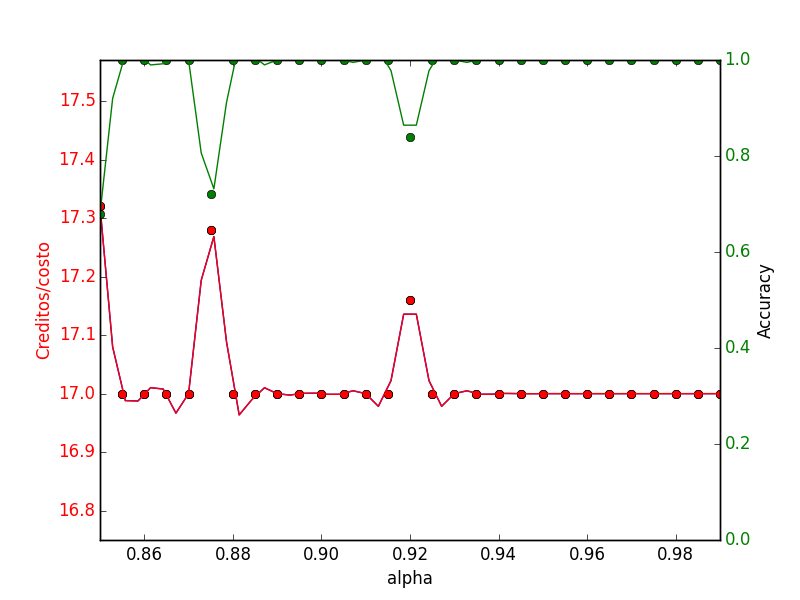
\includegraphics[width=\linewidth]{img/1-alpha-bacp8.png}
        \caption{Variación de $\alpha$ en bacp8}
        \label{fig:alpha1}
    \endminipage\hfill
    \minipage{0.33\textwidth}
        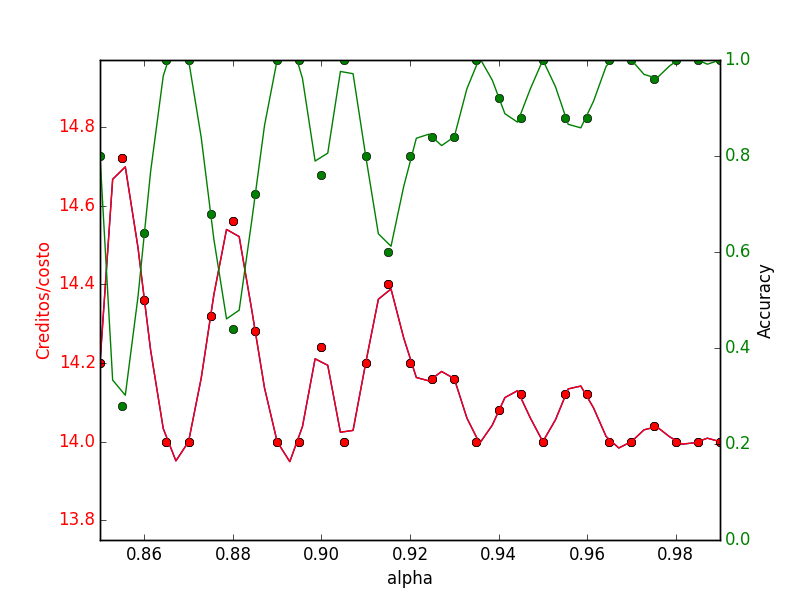
\includegraphics[width=\linewidth]{img/1-alpha-bacp10.png}
        \caption{Variación de $\alpha$ en bacp10}
        \label{fig:alpha2}
    \endminipage\hfill
    \minipage{0.33\textwidth}%
    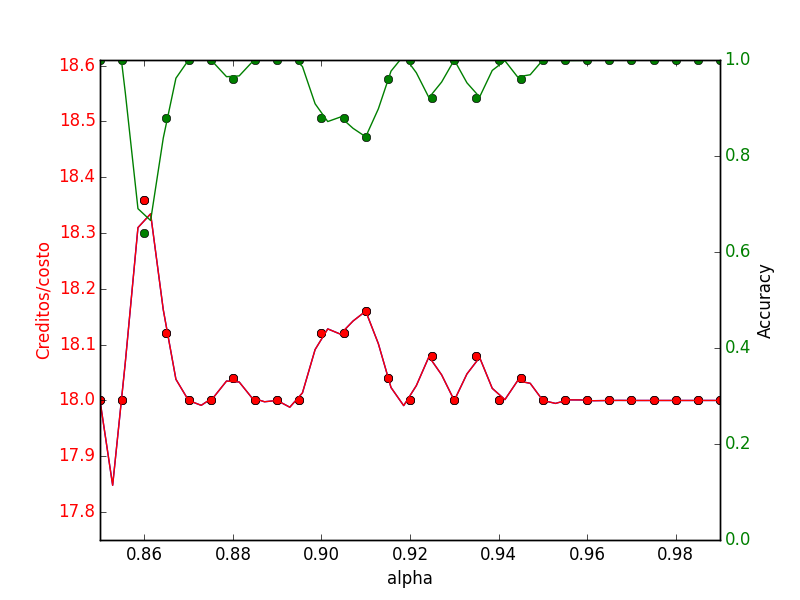
\includegraphics[width=\linewidth]{img/1-alpha-bacp12.png}
        \caption{Variación de $\alpha$ en bacp12}
        \label{fig:alpha3}
    \endminipage
\end{figure}

Con los siguientes valores promedios:

\begin{table}[H]
  \centering
  \begin{tabular}{@{}lcccc@{}}
    \toprule[1pt]
    Instancia & Tiempo & Carga & Accuracy Promedio & Accuracy Final \\
    \midrule
     bacp8 & 0.3705 [s] & 17.0262 [crédito] & 97.3793\% & 99.8461\% \\
    bacp10 & 0.3398 [s] & 14.1476 [crédito] & 85.2414\% & 98.9567\% \\
    bacp12 & 0.7599 [s] & 18.0400 [crédito] & 96.0000\% & 99.7782\% \\
    \bottomrule
  \end{tabular}
  \caption{Valores promedios de SA + Greedy sobre bacp8, bacp10 y bacp12 variando $\alpha$}
\end{table}

Observando los tres graficos se aprecia que mientras mayor es $\alpha$, mayor cantidad de interaciones de temperatura SA debe realizar, por lo que se nota la tendencia a obtener una exactitud del 100\% cerca de un $\alpha = 0.93$ en adelante. Los únicos puntos anormales son el 0.85, 0.875, 0.92 los cuales presentaron un promedio de 17.25 créditos en las 25 repeticiones de la instancia en cada punto.

En este caso del bacp10 se comporto de manera mas errática, pero con una clara tendencia a llegar a los 14 créditos a medida que $\alpha$ aumenta. Nuevamente se observa que los puntos 0.85, 0.875 y 0.92 tienen un peor rendimiento en encontrar el óptimo.

Para el bacp12 el comportamiento fue similar al bacp8, un poco mas violento hasta antes del 0.95 pero la tendencia a estabilizarse es la misma y termina con una exactitud cercana 100\%.

Con respecto a los tiempos promedios, tanto el bacp8 como el bacp10 les tomo solo 0.35 [s] en encontrar soluciones, mientras que el bacp12 fue de cerca del 0.7 [s], aproximadamente el doble de tiempo. Sin embargo la peor exactitud fue la entregada por bacp10, con un 85\% promedio, mientras que bacp8 y bacp12 están ambas por sobre el 95\% de exactitud promedio. De todas formas las exactitudes totales de todas las instancias fueron superiores al 98\%.

\subsection{Experimento 2: Iteraciones locales}

Los resultados obtenidos tras 825 ejecuciones, 275 por cada problema bacp8, bacp10 y bacp12 variando unicamente el parametro \texttt{iter} y dejando todo lo demás constante como:

\begin{description}
    \item[$\alpha$:] 0.90
    \item[t-init:] 1.0
    \item[t-min:] 0.00001
\end{description}
Se obtuvieron los siguientes resultados

\begin{figure}[H]
    \minipage{0.33\textwidth}
        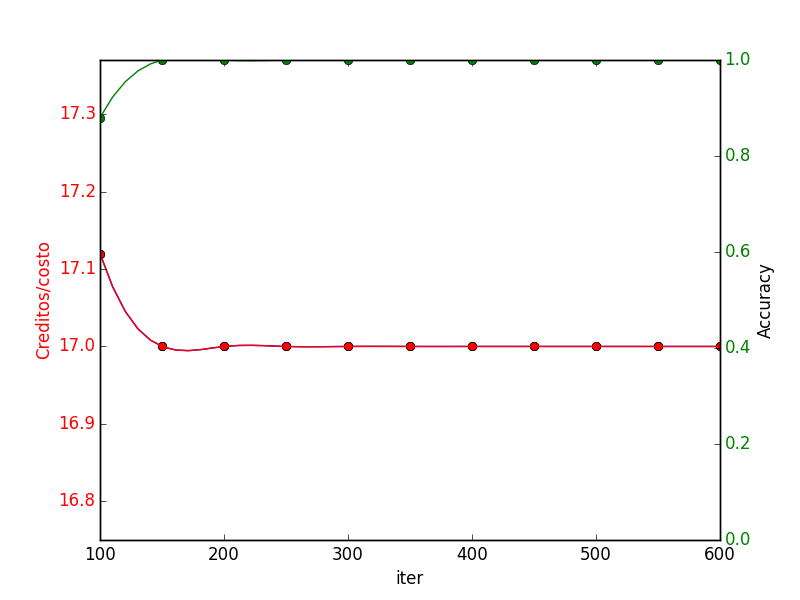
\includegraphics[width=\linewidth]{img/2-iter-bacp8.png}
        \caption{Variación de iteraciones locales en bacp8}
        \label{fig:iter1}
    \endminipage\hfill
    \minipage{0.33\textwidth}
        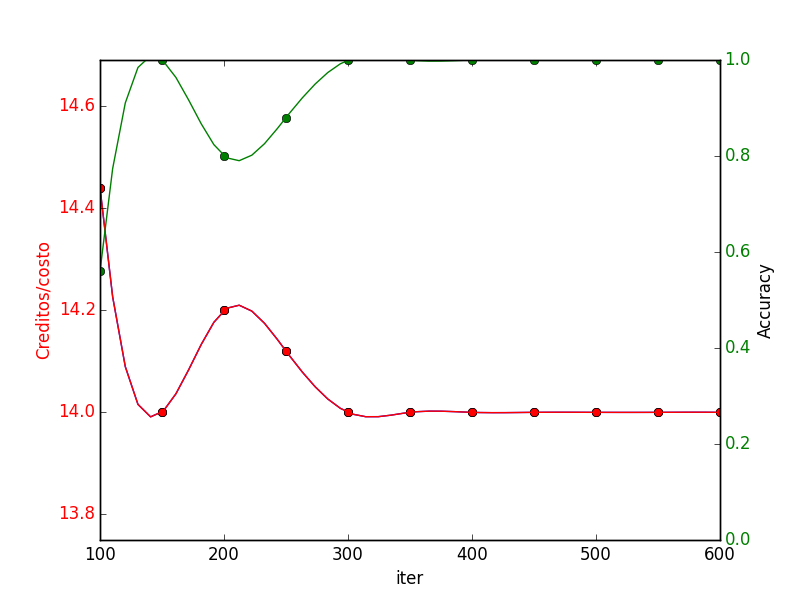
\includegraphics[width=\linewidth]{img/2-iter-bacp10.png}
        \caption{Variación de iteraciones locales en bacp10}
        \label{fig:iter2}
    \endminipage\hfill
    \minipage{0.33\textwidth}%
    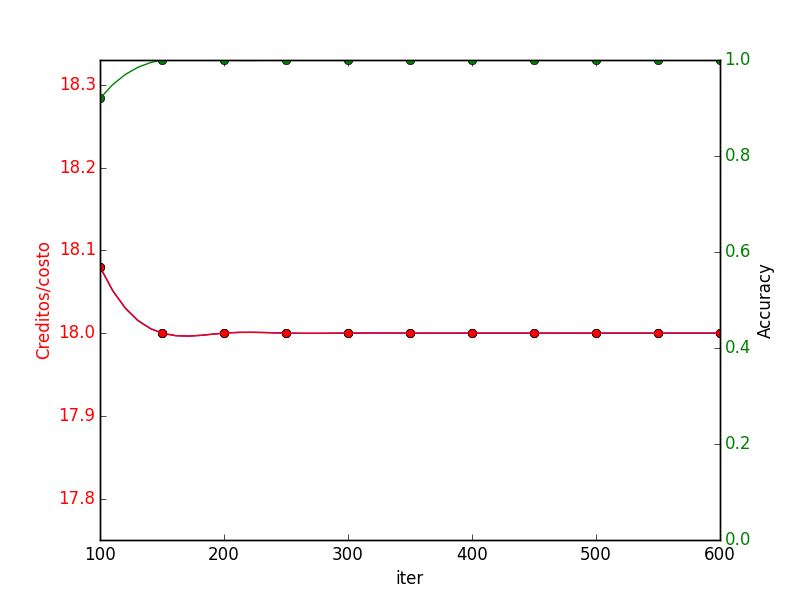
\includegraphics[width=\linewidth]{img/2-iter-bacp12.png}
        \caption{Variación de iteraciones locales en bacp12}
        \label{fig:iter3}
    \endminipage
\end{figure}

Con los siguientes valores promedios:

\begin{table}[H]
  \centering
  \begin{tabular}{@{}lcccc@{}}
    \toprule[1pt]
    Instancia & Tiempo & Carga & Accuracy Promedio & Accuracy Final \\
    \midrule
     bacp8 &  0.6107 [s] & 17.0109 [crédito] &  98.9090\% & 99.9359\% \\
    bacp10 &  0.5700 [s] & 14.0691 [crédito] &  93.0910\% & 99.5089\% \\
    bacp12 & 1.25711 [s] & 18.0073 [crédito] &  99.2730\% & 99.9595\% \\
    \bottomrule
  \end{tabular}
  \caption{Valores promedios de SA + Greedy sobre bacp8, bacp10 y bacp12 variando \texttt{iter}}
\end{table}

Lo primero que se observa en este experimento es que los valores se llega rápidamente a soluciones optimas a medida que la cantidad de iteraciones locales aumenta. Incluso en la instancia bacp10, la cual en el experimento anterior resulto ser la mas errática, en este caso solo tiene los valores 100, 200 y 250 incorrectos, ya a partir de las 300 iteraciones logra llegar casi siempre al optimo.

Por otro lado las instancias bacp8 y bacp12 tienen un comportamiento muy similar, con tan solo 150 iteraciones en adelante se obtienen resultados óptimos. La diferencia entre ambos se produce en el tiempo de ejecución, bacp12 le toma el doble de tiempo que a bacp8. Resalta la exactitud promedio de un 99\% en ambos casos, y de casi el 100\% en la exactitud total.

bacp10 es el único que tuvo menor exactitud promedio de 93.091\%, pero aun así fue mejor que en el experimento 1 donde solo obtuvo un 85.2414\%.

Cabe resaltar que en este experimento se esta utilizando el mejor valor encontrado para $\alpha$ en el experimento 1. Lo suficientemente bueno como para entregar resultados significativos, pero que a su vez no sea demasiado costoso de ejecutar. Se opto por usar el 0.9 para $\alpha$.





\subsection{Experimento 3: Temperatura}

Los resultados obtenidos tras 375 ejecuciones, 125 por cada problema bacp8, bacp10 y bacp12 variando unicamente el parametro \texttt{t-min} y dejando todo lo demás constante como:

\begin{description}
    \item[$\alpha$:] 0.90
    \item[iter:] 250
    \item[t-init:] 1.0
\end{description}
Se obtuvieron los siguientes resultados

\begin{figure}[H]
    \minipage{0.33\textwidth}
        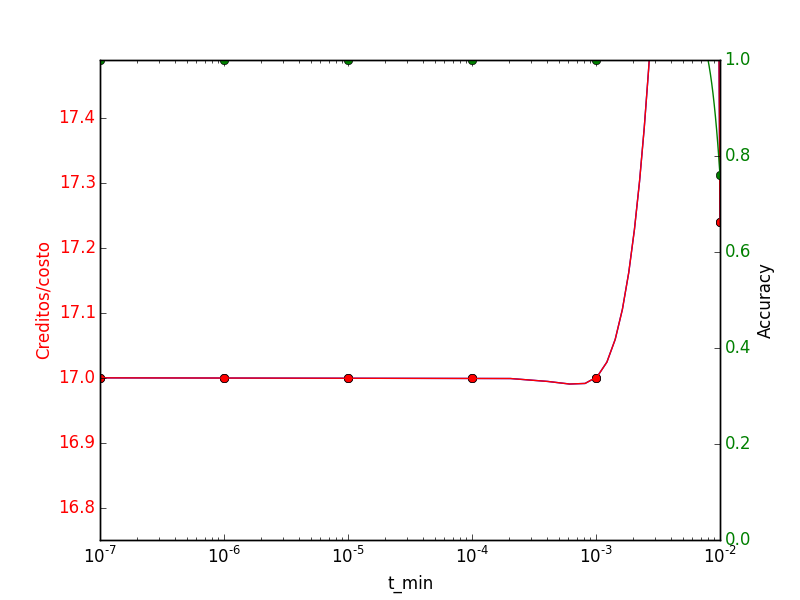
\includegraphics[width=\linewidth]{img/3-tmin-bacp8.png}
        \caption{Variación de temperatura mínima en bacp8}
        \label{fig:tmin1}
    \endminipage\hfill
    \minipage{0.33\textwidth}
        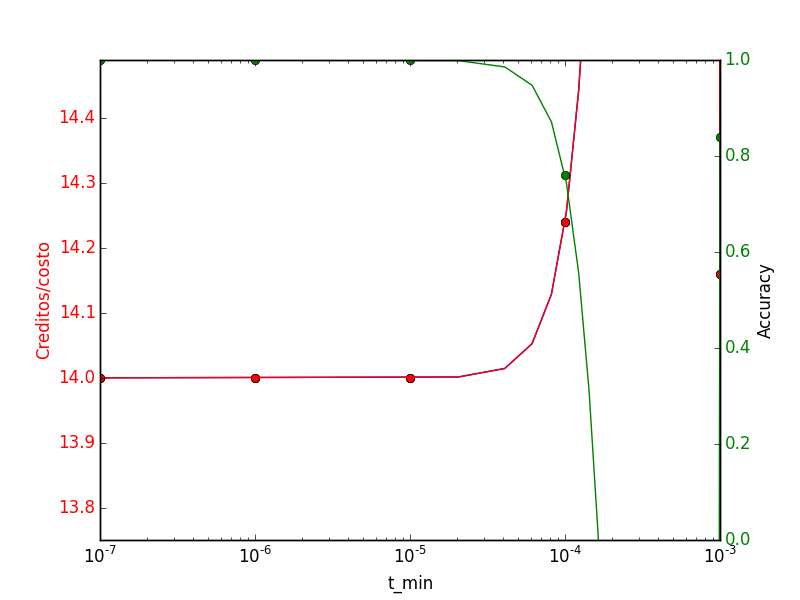
\includegraphics[width=\linewidth]{img/3-tmin-bacp10.png}
        \caption{Variación de temperatura mínima en bacp10}
        \label{fig:tmin2}
    \endminipage\hfill
    \minipage{0.33\textwidth}%
    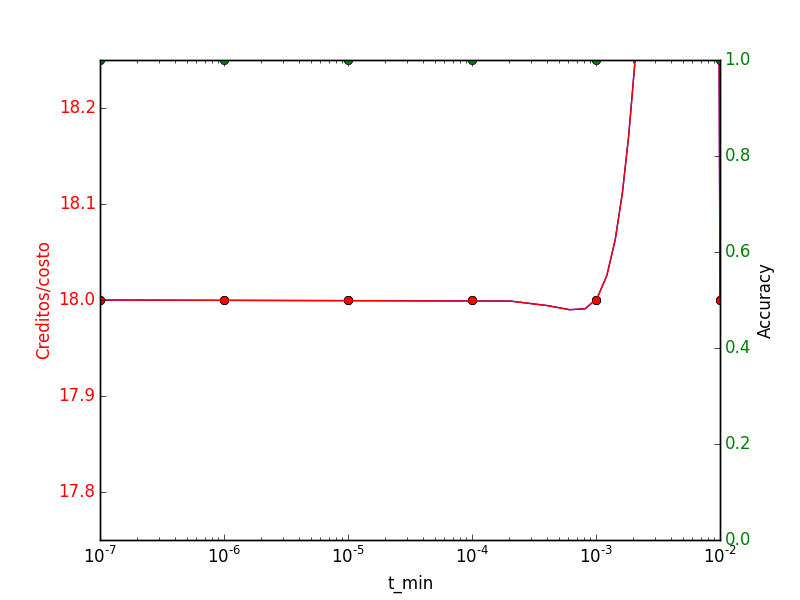
\includegraphics[width=\linewidth]{img/3-tmin-bacp12.png}
        \caption{Variación de temperatura mínima en bacp12}
        \label{fig:tmin3}
    \endminipage
\end{figure}

Con los siguientes valores promedios:

\begin{table}[H]
  \centering
  \begin{tabular}{@{}lcccc@{}}
    \toprule[1pt]
    Instancia & Tiempo & Carga & Accuracy Promedio & Accuracy Final \\
    \midrule
     bacp8 &  0.3882 [s] & 17.0400 [crédito] &   96.0000\% &  99.7653\% \\
    bacp10 &  0.4219 [s] & 14.0800 [crédito] &   92.0000\% &  99.5089\% \\
    bacp12 &  0.7914 [s] & 18.0000 [crédito] &  100.0000\% & 100.0000\% \\
    \bottomrule
  \end{tabular}
  \caption{Valores promedios de SA + Greedy sobre bacp8, bacp10 y bacp12 variando \texttt{iter}}
\end{table}

En este experimento el gráfico se lee al revés, los valores mas pequeños para \texttt{t\_min} representan una mayor iteración de temperaturas, por lo que los resultados deberían acercarse mejor a una solución óptima. La temperatura mínima esta en escala logarítmica.

Nuevamente bacp8 y bacp12 tienen un comportamiento muy similar, solo fallan en el orden de los $10^{-2}$, ya desde los $10^{-3}$ logran llegar a soluciones optimas siempre. bacp10 solo logra estabilizarse al llegar al orden de los $10^{-5}$.

En este experimento se utilizan los mejores parámetros de los dos experimentos anteriores, $\alpha = 0.90$ y \texttt{iter} = 250. Por lo que la calidad del experimento actual debiese ser superior. Los tiempos de ejecución para el bacp8 y bacp10 están cerca de los 0.4 [s] mientras que nuevamente bacp12 llega al doble con 0.4 [s]. Este parece ser un patron recurrente en todos los experimentos, bacp8 y bacp10 toman tiempos similares mientras que bacp12 toma el doble de tiempo. El otro patrón recurrente es el comportamiento similar entre bacp8 y bacp12, pues suelen poseer para los mismos parámetros resultados similares.

Con respecto a las exactitudes es notable el 100\% obtenido en la instancia bacp12, muy de cerca bacp8 y nuevamente bacp10 resulta ser el que posee menor exactitud con un 92\%.



\section{Conclusiones}

% Conclusiones RELEVANTES del estudio realizado. Debería contener conclusiones
% del informe 1 junto con conclusiones obtenidas del desarrollo del
% software, análisis de resultados de experimentos y trabajo futuro.
En este informe se presentó el estado del arte sobre el problema BACP. Se resumió la evolución en los métodos que han surgido para resolver este problema. Una de las mejores formas de resolver este problema consiste en utilizar métodos híbridos utilizando heurísticas inteligentes con búsquedas locales (Simulated annealing, Tabu Search y Dynamic Tabusearch)~\cite{GbacpGaspero} que permiten guiar a los algoritmos a resultados óptimos rápidamente.

Dentro de los posibles modelos, el criterio de minimización del máximo de las cargas de todos los periodos permite resolver el problema, no es el mas óptimo para diferenciar soluciones. El criterio de minimización de distancias medias propuesto en~\cite{Monette07acp} resulta ser mas eficaz al momento de generar distintas soluciones.

Estos nuevos modelos y técnicas híbridas dan la posibilidad a la aparición de variantes mas complejas como lo es el GBACP propuesto en~\cite{GbacpGaspero,balac}.

Como futuras líneas de investigación sería interesante ver el comportamiento de otras técnicas completas, la mayoría utilizan híbridos de locales con CP. Quizás probar con Backtracking  o Forward Checking a pesar de los grandes espacios de búsqueda. Por otra parte se demostró que los métodos híbridos son un buen acercamiento para resolver este problema, sería interesante realizar nuevas mezclas híbridas por ejemplo GA con búsquedas locales como Tabu Search o Simulated Annealing.

\section{Bibliografía}

Indicando toda la información necesaria de acuerdo al tipo de documento
revisado. Las referencias deben ser citadas en el documento.  \bibliographystyle{plain}
\bibliography{Referencias}

\end{document}
